\chapter{Bab 3}

\section{Identasi}
Identasi adalah penulisan paragraf yang agak menjorok masuk ke dalam (tab atau spasi 2x/4x). di analisa saya hanya satu yang ditemukan yaitu ketika source code ditulis secara satu garis lurus. untuk error ada di iphyton console. ketika di run aplikasi tidak bisa dijalan kan dan ada tulisan IndentationError : expected indent block. yang berarti baris paragraf terhalang. posisi errornya juga diberi tahu dengan muncul notif peringatan kuning dan no line yang error di ipython console. berikut gambar yang sebelum diperbaiki dan sesudah diperbaiki.
\begin{figure}[H]
	\centering
	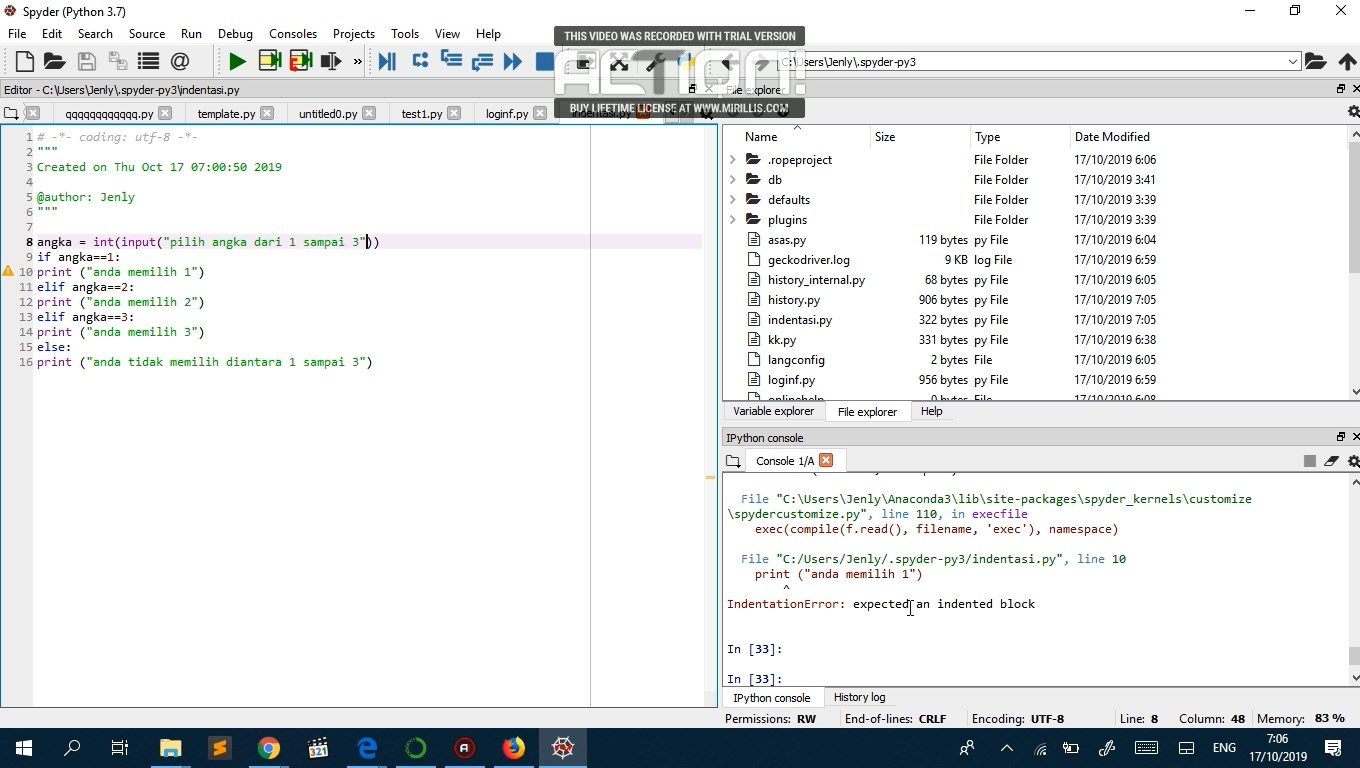
\includegraphics[width=8cm]{figures/a1.jpg}
\end{figure}

\begin{figure}[H]
	\centering
	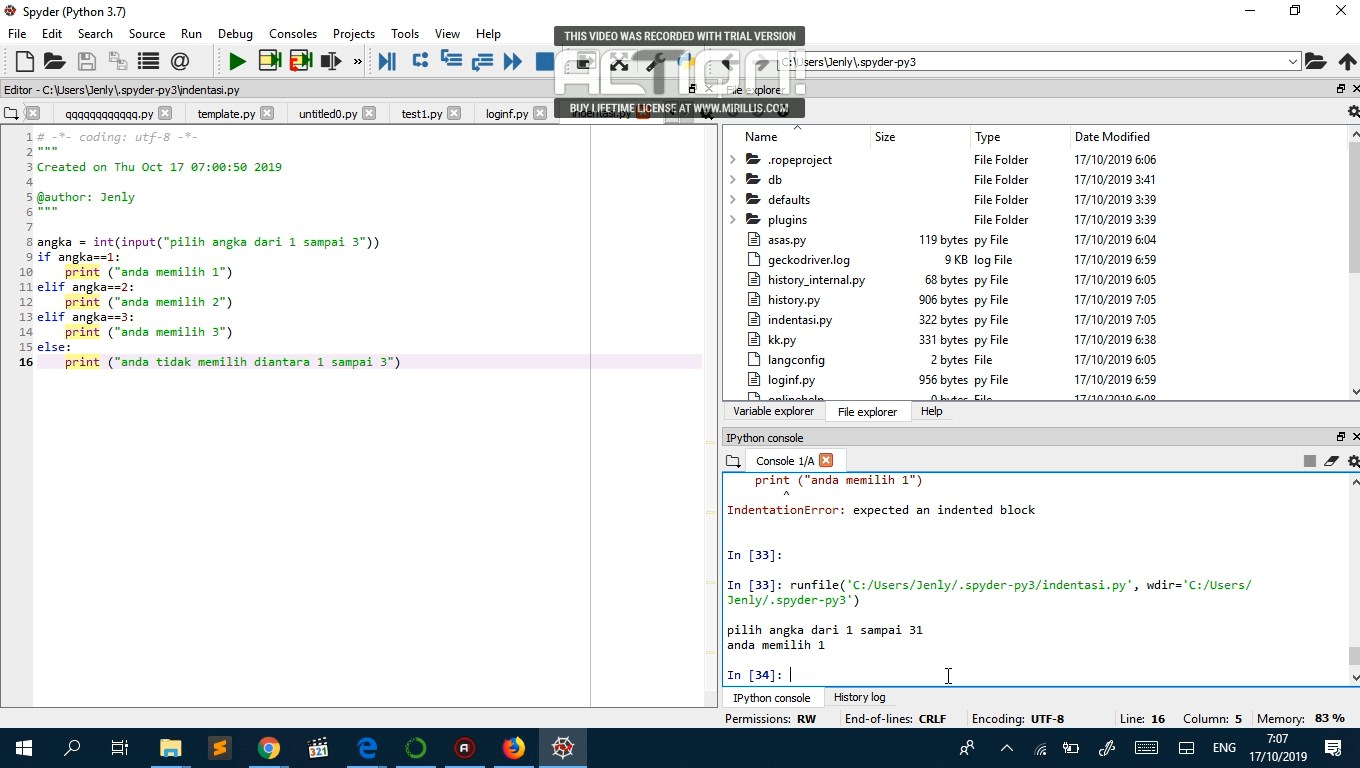
\includegraphics[width=8cm]{figures/a2.jpg}
\end{figure}
